%  LaTeX support: latex@mdpi.com 
%  In case you need support, please attach all files that are necessary for compiling as well as the log file, and specify the details of your LaTeX setup (which operating system and LaTeX version / tools you are using).

% You need to save the "mdpi.cls" and "mdpi.bst" files into the same folder as this template file.

%=================================================================
\documentclass[journal,article,submit,moreauthors,pdftex,10pt,a4paper]{mdpi} 
%
%--------------------
% Class Options:
%--------------------
% journal
%----------
% Choose between the following MDPI journals:
% actuators, addictions, admsci, aerospace, agriculture, agronomy, algorithms, animals, antibiotics, antibodies, antioxidants, applsci, arts, asi, atmosphere, atoms, axioms, batteries, bdcc, behavsci, beverages, bioengineering, biology, biomedicines, biomimetics, biomolecules, biosensors, brainsci, buildings, carbon, cancers, catalysts, cells, ceramics, challenges, chemengineering, chemosensors, children, chromatography, climate, coatings, colloids, computation, computers, condensedmatter, cosmetics, cryptography, crystals, cybersecurity, data, dentistry, designs, diagnostics, diseases, diversity, econometrics, economies, education, electrochemistry, electronics, energies, entropy, environments, epigenomes, est, fermentation, fibers, fire, fishes, fluids, foods, forests, fractalfract, futureinternet, galaxies, games, gastrointestdisord, gels, genealogy, genes, geosciences, geriatrics, hazardousmatters, healthcare, heritage, highthroughput, horticulturae, humanities, hydrology, informatics, information, infrastructures, inorganics, insects, instruments, ijerph, ijfs, ijms, ijgi, ijtpp, inventions, j, jcdd, jcm, jcs, jdb, jfb, jfmk, jimaging, jof, jintelligence, jlpea, jmmp, jmse, jpm, jrfm, jsan, land, languages, laws, life, literature, logistics, lubricants, machines, magnetochemistry, make, marinedrugs, materials, mathematics, mca, mti, medsci, medicines, membranes, metabolites, metals, microarrays, micromachines, microorganisms, minerals, modelling, molbank, molecules, mps, nanomaterials, ncrna, neonatalscreening, nitrogen, nutrients, ohbm, particles, pathogens, pharmaceuticals, pharmaceutics, pharmacy, philosophies, photonics, plants, plasma, polymers, preprints, proceedings, processes, proteomes, publications, quaternary, qubs, recycling, religions, remotesensing, resources, risks, robotics, safety, scipharm, sensors, separations, sexes, sinusitis, socsci, societies, soils, sports, standards, surgeries, sustainability, symmetry, systems, technologies, toxics, toxins, tropicalmed, universe, urbansci, vaccines, vetsci, vibration, viruses, vision, water, wem
%---------
% article
%---------
% The default type of manuscript is article, but can be replaced by: 
% abstract, addendum, article, benchmark, book, bookreview, briefreport, casereport, changes, comment, commentary, communication, conceptpaper, correction, conferenceproceedings, conferencereport, expressionofconcern, meetingreport, creative, datadescriptor, discussion, editorial, essay, erratum, hypothesis, interestingimages, letter, meetingreport, newbookreceived, opinion, obituary, projectreport, reply, reprint, retraction, review, perspective, protocol, shortnote, supfile, technicalnote, viewpoint
% supfile = supplementary materials
% protocol: If you are preparing a "Protocol" paper, please refer to http://www.mdpi.com/journal/mps/instructions for details on its expected structure and content.
%----------
% submit
%----------
% The class option "submit" will be changed to "accept" by the Editorial Office when the paper is accepted. This will only make changes to the frontpage (e.g. the logo of the journal will get visible), the headings, and the copyright information. Also, line numbering will be removed. Journal info and pagination for accepted papers will also be assigned by the Editorial Office.
%------------------
% moreauthors
%------------------
% If there is only one author the class option oneauthor should be used. Otherwise use the class option moreauthors.
%---------
% pdftex
%---------
% The option pdftex is for use with pdfLaTeX. If eps figures are used, remove the option pdftex and use LaTeX and dvi2pdf.

%=================================================================
\firstpage{1} 
\makeatletter 
\setcounter{page}{\@firstpage} 
\makeatother 
\articlenumber{x}
\doinum{10.3390/------}
\pubvolume{xx}
\pubyear{2017}
\copyrightyear{2017}
\externaleditor{Academic Editor: name}
\history{Received: date; Accepted: date; Published: date}

%------------------------------------------------------------------
% The following line should be uncommented if the LaTeX file is uploaded to arXiv.org
%\pdfoutput=1

%=================================================================
% Add packages and commands here. The following packages are loaded in our class file: fontenc, calc, indentfirst, fancyhdr, graphicx, lastpage, ifthen, lineno, float, amsmath, setspace, enumitem, mathpazo, booktabs, titlesec, etoolbox, amsthm, hyphenat, natbib, hyperref, footmisc, geometry, caption, url, mdframed, tabto, soul, multirow, microtype, tikz

%=================================================================
%% Please use the following mathematics environments: Theorem, Lemma, Corollary, Proposition, Characterization, Property, Problem, Example, ExamplesandDefinitions, Hypothesis, Remark, Definition
%% For proofs, please use the proof environment (the amsthm package is loaded by the MDPI class).

%=================================================================
% Full title of the paper (Capitalized)
\Title{Creation of Braille plates using 3D printing technology}

% Author Orchid ID: enter ID or remove command
\newcommand{\orcidauthorA}{0000-0000-000-000X} % Add \orcidA{} behind the author's name
%\newcommand{\orcidauthorB}{0000-0000-000-000X} % Add \orcidB{} behind the author's name

% Authors, for the paper (add full first names)
\Author{Vasilij Konstantinov $^{1,\dagger,\ddagger}$\orcidA{}, Orlova Yuilia $^{1,\ddagger}$ and Vladimir Rozaliev $^{2,}$*}

% Authors, for metadata in PDF
\AuthorNames{Vasilij Konstantinov, Orlova Yuilia and Vladimir Rozaliev}

% Affiliations / Addresses (Add [1] after \address if there is only one affiliation.)
\address{%
$^{1}$ \quad Affiliation 1; konstantinovr1@gmail.com\\
$^{2}$ \quad Affiliation 2; yulia.orlova@gmail.com}

% Contact information of the corresponding author
\corres{Correspondence: vladimir.rozaliev@gmail.com; Tel.: +7-917-336-69-88}

% Current address and/or shared authorship
\firstnote{Current address: vladimir.rozaliev@gmail.com} 
\secondnote{These authors contributed equally to this work.}
% The commands \thirdnote{} till \eighthnote{} are available for further notes

% Simple summary
%\simplesumm{}

% Abstract (Do not insert blank lines, i.e. \\) 
\abstract{This article describes a program for the printing Braille tables using 3D printer. A basic function is creation the STL file containing Braille tables geometrical characteristics which representing input text. The received out-put file can print on the 3D printer.}

% Keywords
\keyword{Braille plates; 3D printing}

% The fields PACS, MSC, and JEL may be left empty or commented out if not applicable
%\PACS{J0101}
%\MSC{}
%\JEL{}

%%%%%%%%%%%%%%%%%%%%%%%%%%%%%%%%%%%%%%%%%%
% Only for the journal Applied Sciences:
%\featuredapplication{Authors are encouraged to provide a concise description of the specific application or a potential application of the work. This section is not mandatory.}
%%%%%%%%%%%%%%%%%%%%%%%%%%%%%%%%%%%%%%%%%%

%%%%%%%%%%%%%%%%%%%%%%%%%%%%%%%%%%%%%%%%%%
% Only for the journal Data:
%\dataset{DOI number or link to the deposited data set in cases where the data set is published or set to be published separately. If the data set is submitted and will be published as a supplement to this paper in the journal Data, this field will be filled by the editors of the journal. In this case, please make sure to submit the data set as a supplement when entering your manuscript into our manuscript editorial system.}

%\datasetlicense{license under which the data set is made available (CC0, CC-BY, CC-BY-SA, CC-BY-NC, etc.)}

%\setcounter{secnumdepth}{4}
%%%%%%%%%%%%%%%%%%%%%%%%%%%%%%%%%%%%%%%%%%

\begin{document}
%%%%%%%%%%%%%%%%%%%%%%%%%%%%%%%%%%%%%%%%%%
%% Only for the journal Gels: Please place the Experimental Section after the Conclusions

%%%%%%%%%%%%%%%%%%%%%%%%%%%%%%%%%%%%%%%%%%
\setcounter{section}{0} %% Remove this when starting to work on the template.

\section{Introduction}

Braille is named after its creator, Frenchman Louis Braille, who lost his eyesight due to a childhood accident. In 1824, at the age of 15, Braille developed his code for the French alphabet as an improvement on night writing. He published his system, which subsequently included musical notation, in 1829. The second revision, pub-lished in 1837, was the first binary form of writing developed in the modern era[1].
Braille characters are small rectangular blocks called cells that contain tiny pal-pable bumps called raised dots. The number and arrangement of these dots distin-guish one character from another. Since the various braille alphabets originated as transcription codes of printed writing systems, the mappings (sets of character des-ignations) vary from language to language.
Braille is derived from the Latin alphabet, albeit indirectly. In Braille's original system, the dot patterns were assigned to letters according to their position within the alphabetic order of the French alphabet. The first ten letters of the alphabet, a–j, use the upper four dot positions. These stand for the ten digits 1–9 and 0 in a system parallel to Hebrew gematria and Greek isopsephy. (Though the dots are assigned in no obvious order, the cells with the fewest dots are assigned to the first three letters (and lowest digits), a-b-c = 1-2-3, and to the three vowels in this part of the alphabet, a-e-i, whereas the even digits, 4, 6, 8, 0 are corners/right angles.) The next ten letters, k–t, are identical to a–j, respectively, apart from the addition of a dot at position 3 (red dots in the table). Figure 1 represents a braille alphabet.

\begin{figure}[H]
\centering
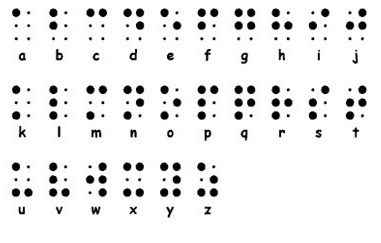
\includegraphics[width=10 cm]{Braiile-Alphabet.jpg}
\caption{Braille alphabet showing arrangement of dots that make up each letter. Note: the little dots are placeholders and are not to be printed.}
\end{figure} 
 
%%%%%%%%%%%%%%%%%%%%%%%%%%%%%%%%%%%%%%%%%%
\section{Description of the building STL file method}

For the printing of the Braille book, consisting of tables on the 3D printer it is necessary to create at first the file containing spatial characteristics of this table. As the technology of the printing by a fusing method is at the moment most developed and available (Fused deposition modeling, FDM) in which an object is created by layerwise laying down of the melted thread of melting working material (plastic, metal, wax), we will save spatial characteristics in the STL file. The description of each edge begins with the keyword of "facet". Further there is a description of a normal to this edge in the form of a vector with three coordinates. The description of a normal begins with the word "normal". Further there is a unit of the description of peaks of the edge. This unit is framed with the words "outer loop" and "endloop". In the unit each peak of a triangular edge is described by three spatial coordinates. The unit of the description of an edge comes to an end with the word "endfacet"[3].
Thus, it is possible to select the principal function of the program for the printing of tables of Braille – creation of the STL file containing characteristics of a table of Braille in the input text. Generally, the analysis of the input text comes down to symbol-by-symbol analysis. However, for example, in the English Braille language some words and combinations of words can have special abbreviations. For example, the word "afternoon" in the Braille representation registers as a string of "AFN". At this stage we won't consider these features. Also, we will consider only 6-and a 8-dot font of Braille[2]. Figure 2 shows a Braille dots dimensions schema in the plate.

\begin{figure}[H]
\centering
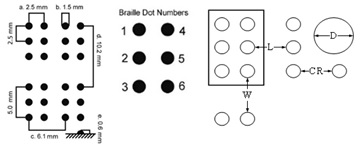
\includegraphics[width=10 cm]{Braille-Dots-Schema.jpg}
\caption{Braille dots dimensions schema}
\end{figure} 

The general diagram of a method::
\begin{enumerate}[leftmargin=*,labelsep=4.9mm]
\item	Symbol-by-symbol analysis of the input text (characters of the Russian and English alphabet, digits, separators);
\item	Search of compliance of the selected characters with 6-dot glyphs (Braille's characters);
\item Division of glyphs into tables (25 glyphs down and 30 across);
\item	Computation of spatial characteristics (coordinates of X, Y, Z, normals) of glyphs in a table;
\item	Saving the calculated characteristics in the STL file.	
\end{enumerate}

As a result of these steps the file which can be viewed also any three-dimensional packet, for example, in MeshLab will be received.

%%%%%%%%%%%%%%%%%%%%%%%%%%%%%%%%%%%%%%%%%%
\section{Description of a braille plate building method}

This section describes a braille plate building method. Method contains 2 steps: processing the input text and calculation of Braille plates parameters; generating a Braille table 3D representation.

%%%%%%%%%%%%%%%%%%%%%%%%%%%%%%%%%%%%%%%%%%
\subsection{Module of processing the input text and calculation of Braille plates parameters}

We will consider process calculation of characteristics of a glyph in the plate. The Glyph model geometrically consists of 2 types of figures: one parallelepiped and 6 cylinders presenting to camber. But as a result of formation of the plate parallelepipeds of the basis of glyphs will coincide with a parallelepiped of the basis of all plate, for definition of her spatial characteristics the X and Y centers of the bases of cylinders of cambers are enough to calculate coordinates. For calculation of horizontal coordinate of the center of a circle $C_{x}$ of the basis of cambers (points) both on six - and on an eight-fine-molded glyph the following formula is used:
For calculation of vertical coordinate in a six-dot glyph the following formulas are used:
\begin{equation}
\mathnormal{C_{x} = i(L+2D+CR)+(x-1)(CR+D)}
\end{equation}
For calculation of vertical coordinate in a six-dot glyph the following formulas are used:
\begin{equation}
\mathnormal{C_{y} = j(W+3D+2CR)+(y-1)(CR+D)	}
\end{equation}
In eight-dot similarly:
\begin{equation}
\mathnormal{C_{y} = j(W+4D+3CR)+(y-1)(CR+D)	}
\end{equation}
where i, j – an index of the calculated camber of a glyph, x, y – a position of camber of a glyph, L – distance between glyphs across, W – distance between glyphs down, CR – distance between the bases glyph circles, D – diameter of the basis of a circle of a glyph.
At the output of the module will create the SVG file which contains visual representation of one plate of Braille and the file with parameters of this plate. The file of parameters of the plate comprises all necessary data (length, width and height of the basis of the plate, height and radius of a circle of the basis of cambers, coordinates of the centers of circles of the bases of cambers) for creation of the STL file.

%%%%%%%%%%%%%%%%%%%%%%%%%%%%%%%%%%%%%%%%%%
\subsection{Module for generating a Braille table 3D representation}

On an output the module receives a set of coordinates of centers of the bases re-ceived at the previous stage. As STL stores the description of geometry in the form of a set of edges and normals to them, in this module it is necessary to realize an algorithm of creation of edges (fig. 1). The base of a table is described by a simple parallelepiped. Cylinders of convexities are presented in the form of the correct n-square. The dimensionality of a n-square the more form of convexity is above ap-proaches cylindrical.
On an output the module creates the STL file which contains complete three-dimensional idea of a table for the printing on the 3D printer. 

\begin{figure}[H]
\centering
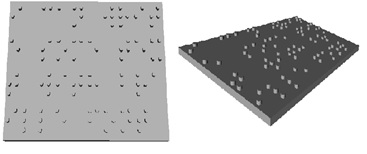
\includegraphics[width=10 cm]{Plate-3D-view.jpg}
\caption{Generated Braille plate representation in MeshLab and printed part of Braille table}
\end{figure} 

The first step is computation of peaks of a circle of the bases of convexities. The circle of the base is presented in the form of the correct n-square where 2 any adjacent peaks divide circle sector into equal angles $\varphi$. This angle is calculated the following on the following formula:

\begin{equation}
\mathnormal{\varphi=\frac{2\pi}{V_{count}}}
\end{equation}

where $V_{count}$ - quantity of peaks of a n-square.

Respectively, coordinates of peak are calculated by the following formula:

\begin{equation}
\mathnormal{X = L_{x} + C_{x} + R\cos\varphi}
\end{equation}

\begin{equation}
\mathnormal{Y = C_{x} + R\sin\varphi}
\end{equation}

\begin{equation}
\mathnormal{Z = const}
\end{equation}

where $R$ - the radius of a circle of the base of convexity, $L_{x}$ – horizontal is long tables.
The second step – to display peak on the upper circle of convexity. As in our representation convexity has the cylindrical form, for display of the base it is enough to increase coordinate $Z$ peaks by convexity height.
The third step is to create from the received edge peaks for formation of STL and to calculate to them normals. Edges of convexities are created as follows. Sequentially two adjacent peaks from the lower base and one, corresponding to one of lower, upper peak are selected. These three selected peaks (A, B, C) create one edge. The normal to this edge is calculated on the following formula:

\begin{equation}
\mathnormal{N_{facet}=(B-A)(C-A)}
\end{equation}

Further calculated is normally normalized by the maximum component on the following formula:

\begin{equation}
\mathnormal{N_{normal}=\frac{N_facet}{Max(N_{x},N_{y},N_{z})}}
\end{equation}

The fourth step – to create table base edges. This step occurs similarly previous for convexities.
As a result we will receive a complete description of geometry of a table in the STL file.

%%%%%%%%%%%%%%%%%%%%%%%%%%%%%%%%%%%%%%%%%%

\section{Results}

The three-dimensional type of the plate is presented in the figure 4.

\begin{figure}[H]
\centering
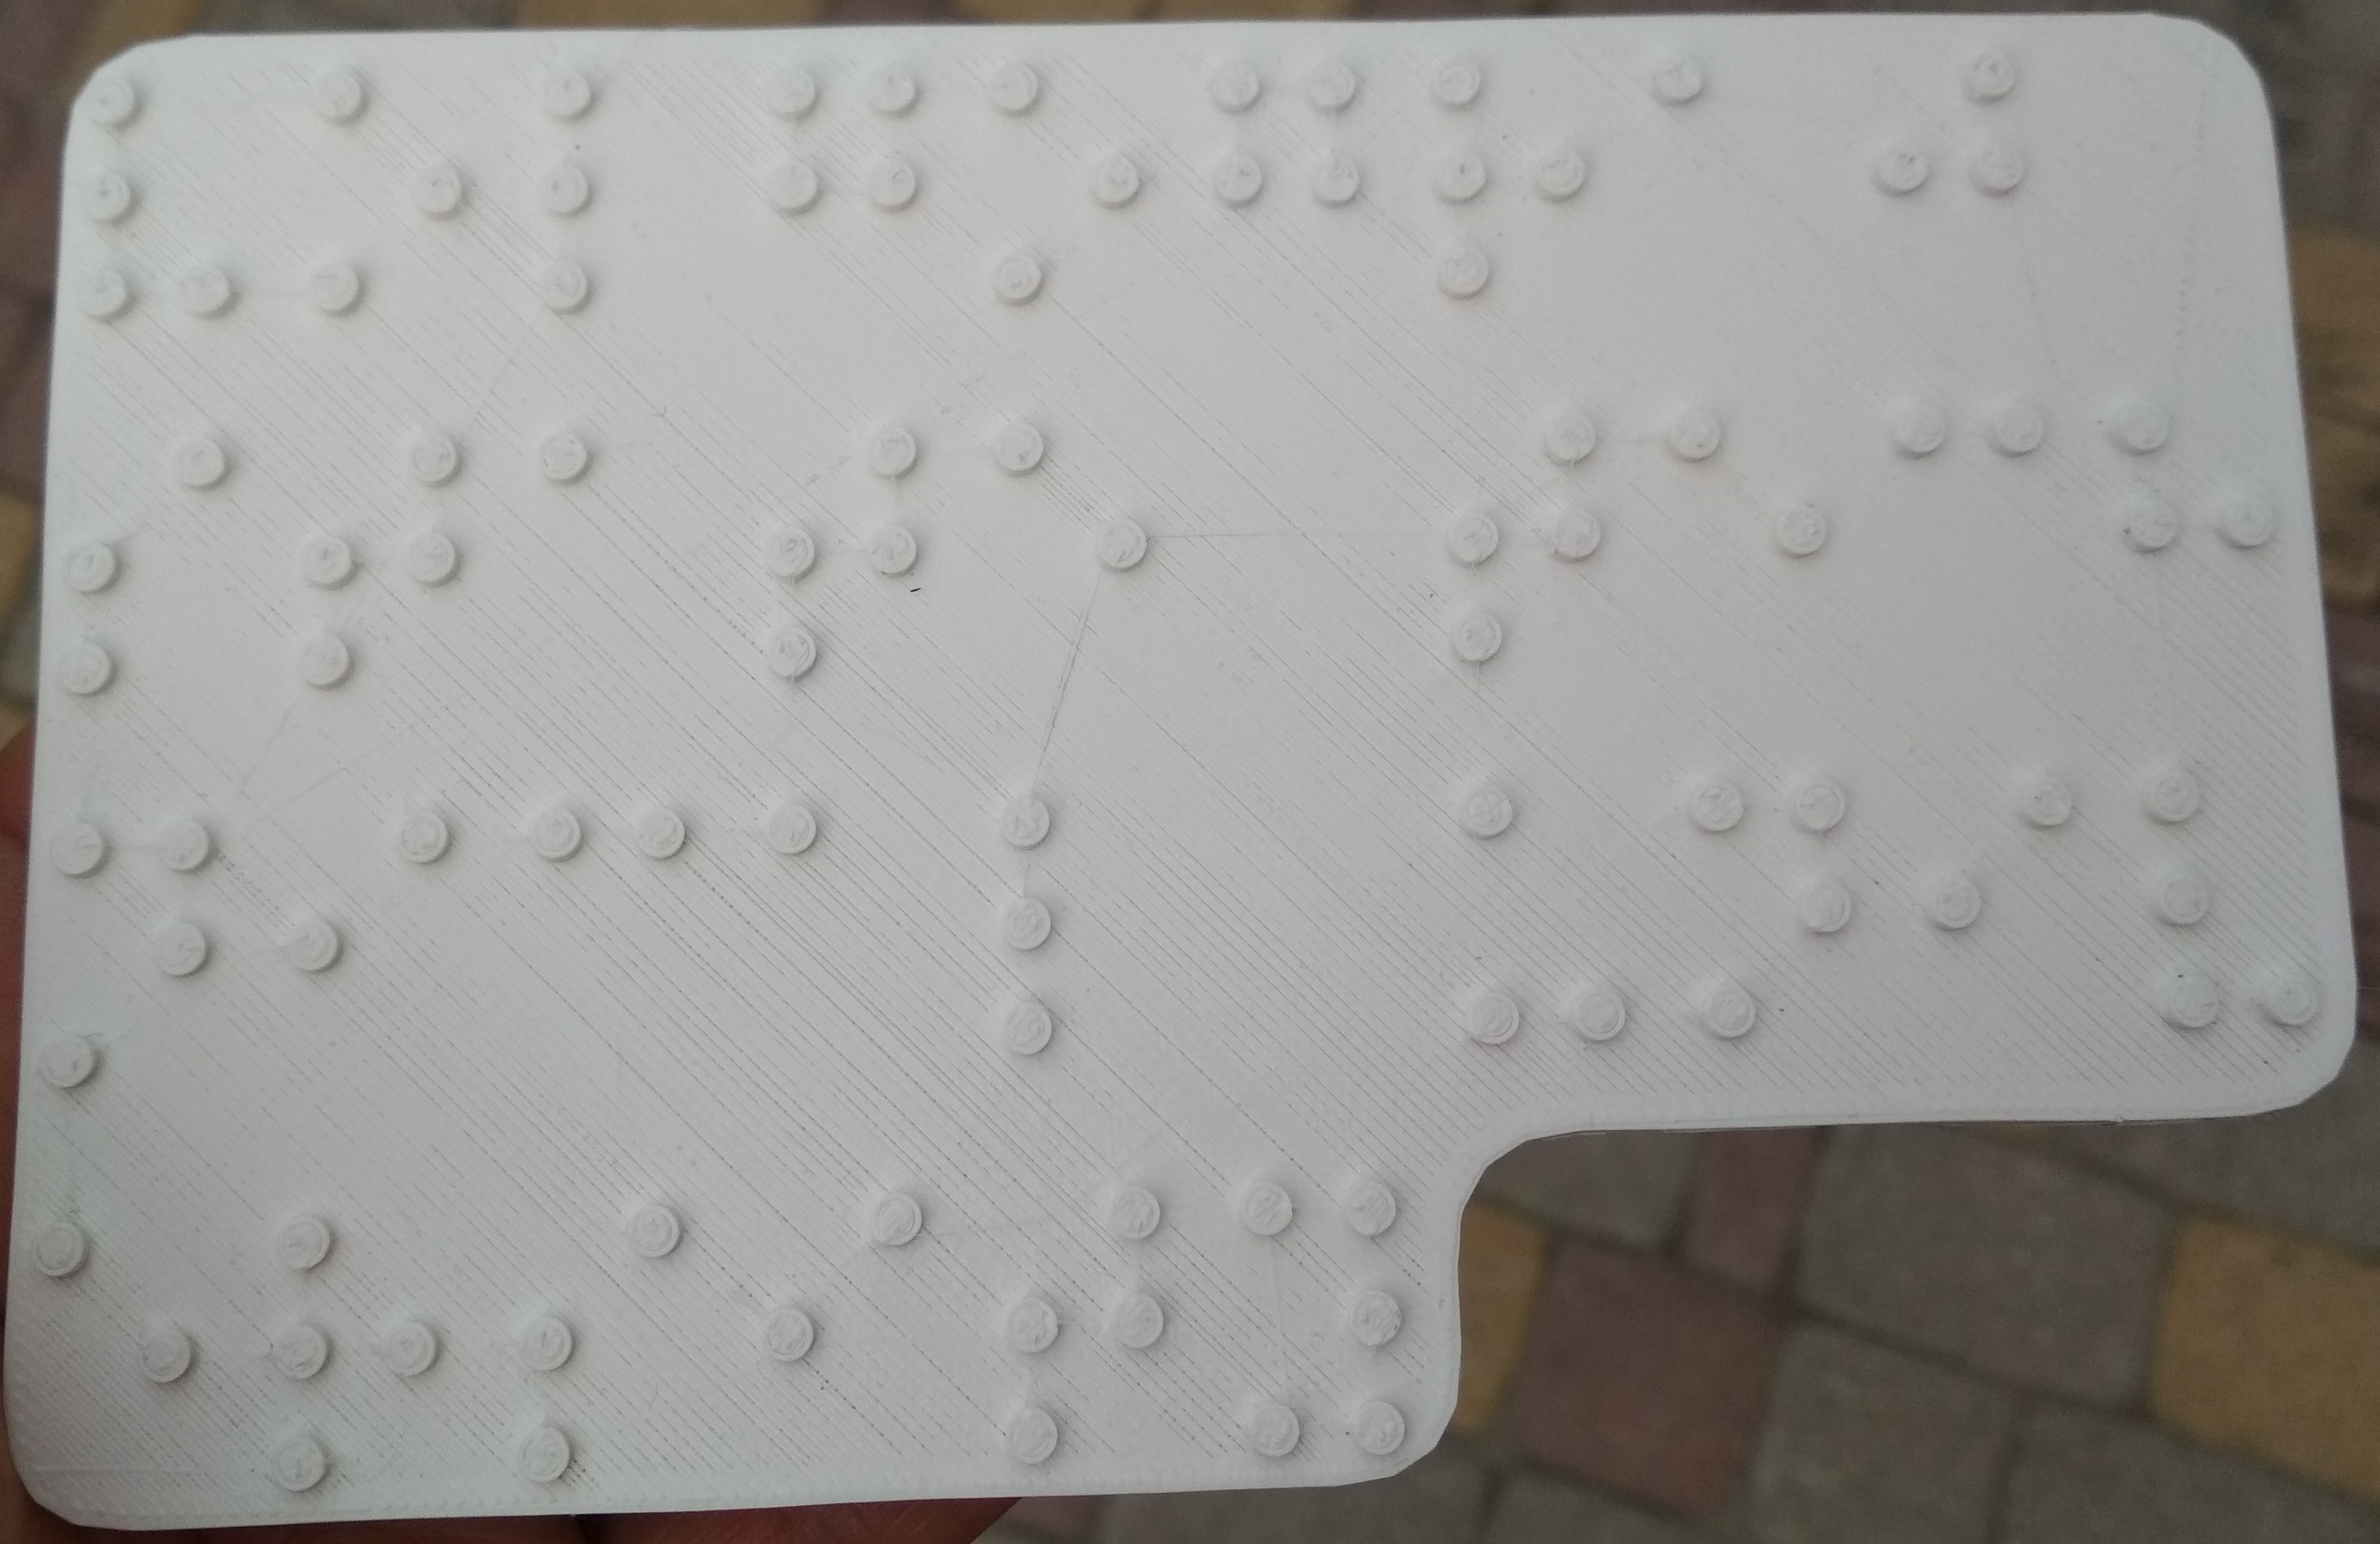
\includegraphics[width=10 cm]{Braille-plate-foto.jpg}
\caption{Printed Braille plate}
\end{figure} 

The developed method of printing of plates of Braille is realized in the form of the program. 

%%%%%%%%%%%%%%%%%%%%%%%%%%%%%%%%%%%%%%%%%%

\section{Discussion}

All defined tasks of this work were successfully complited. 

%%%%%%%%%%%%%%%%%%%%%%%%%%%%%%%%%%%%%%%%%%
\section{Materials and Methods}

STL formation module (language C ++) is github.com/vlusslus/STLGenerator. The module of analysis of the entrance text is github.com/vlusslus/Braille3D.

%%%%%%%%%%%%%%%%%%%%%%%%%%%%%%%%%%%%%%%%%%

\vspace{6pt} 

%%%%%%%%%%%%%%%%%%%%%%%%%%%%%%%%%%%%%%%%%%
% Only for the journal Methods and Protocols:
% If you wish to submit a video article, please do so with any other supplementary material.
% \supplementary{The following are available at www.mdpi.com/link: Figure S1: title, Table S1: title, Video S1: title. A supporting video article is available at doi: link.}

%%%%%%%%%%%%%%%%%%%%%%%%%%%%%%%%%%%%%%%%%%
% Citations and References in Supplementary files are permitted provided that they also appear in the reference list here. 

%=====================================
% References, variant A: internal bibliography
%=====================================
\reftitle{References}
\begin{thebibliography}{999}
% Reference 1
\bibitem[Author1(2016)]
The Dot Positions Are Identified by Numbers from One Through Six. {\em AFB.org} {\bf 2016}, {\em 6}
% Reference 2
\bibitem[Author2(2010)]
Braille. {\em https://en.wikipedia.org/wiki/Braille}
% Reference 3
\bibitem[Author3(2010)]
STL (file format). {\em https://en.wikipedia.org/wiki/STL (file format)}
% Reference 4
\bibitem[Author4(2016)]{ref-journal}
V.M. Konstantinov, V.L. Rozaliev, Y.A. Orlova, A.V. Zaboleeva-Zotova. Development of 3D Human Body Model. {\em Proceedings of the First International Scientific Conference «Intelligent Information Technologies for Industry» (IITI’16)} {\bf 2016}, {\em Vol. 2 / ed. by A. Abraham [etc.]. – [Switzer-land] : Springer International Publishing}, 143-152, Ser. Advances in Intelligent Systems and Computing ; Vol. 451.
\end{thebibliography}

% The following MDPI journals use author-date citation: Arts, Econometrics, Economies, Genealogy, Humanities, IJFS, JRFM, Laws, Religions, Risks, Social Sciences. For those journals, please follow the formatting guidelines on http://www.mdpi.com/authors/references
% To cite two works by the same author: \citeauthor{ref-journal-1a} (\citeyear{ref-journal-1a}, \citeyear{ref-journal-1b}). This produces: Whittaker (1967, 1975)
% To cite two works by the same author with specific pages: \citeauthor{ref-journal-3a} (\citeyear{ref-journal-3a}, p. 328; \citeyear{ref-journal-3b}, p.475). This produces: Wong (1999, p. 328; 2000, p. 475)

%=====================================
% References, variant B: external bibliography
%=====================================
%\externalbibliography{yes}
%\bibliography{your_external_BibTeX_file}

%%%%%%%%%%%%%%%%%%%%%%%%%%%%%%%%%%%%%%%%%%
\end{document}

